\chapter{To POS Tag or Not to POS Tag: The Impact of POS Tags on Morphological Analysis in Low-Resource Settings}
\label{chap:POS}
  

\begin{figure}[tb]
    \centering
    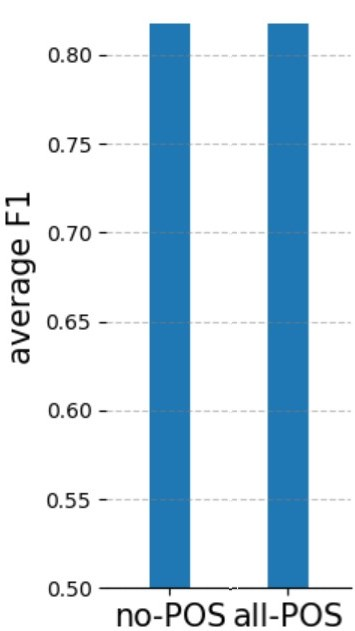
\includegraphics[height=5cm]{figs/POS-avgSegGlossCropped.jpg}
    \hspace{3cm}
    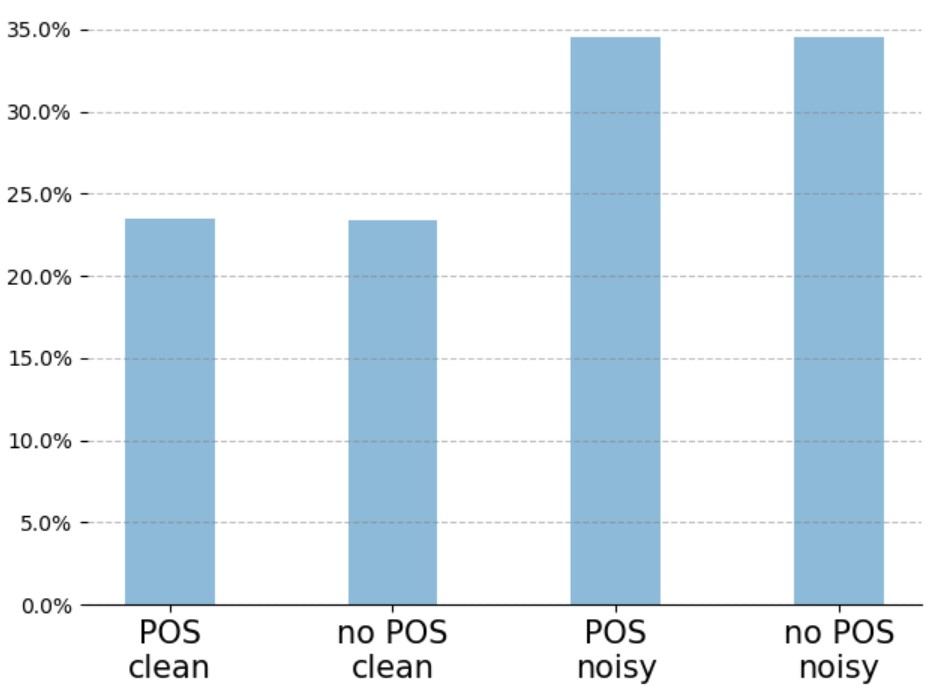
\includegraphics[height=5cm]{figs/POS-avgReinfl.jpg}
    \caption[Comparison of Morphological Tasks with/out POS tags]{Average  F$_1$-scores (right) on joint segmentation and glossing on interlinear glossed texts from fieldwork in five languages found that POS-tags have little and irregular impact. Also, reinflection (left) on four interlinear field corpora and four ``cleaned" versions of those corpora who POS tags make make minimal significant or consistent difference in accuracy.}
    \label{fig:avgseggls}
\end{figure}

Parts of speech (POS), also known as word classes or lexical categories, communicate information about a word, its morphological structure and inflectional paradigm, and its potential grammatical role in a clause. 
%POS tags have been used in NLP work with many languages and 
POS tagging is a well-studied problem in NLP. It is one of the first tasks undertaken for a new data set and a POS tagger is often one of the first NLP resources built for low-resource languages
\citep{yarowsky_inducing_2001,cox_probabilistic_2010,de_pauw_resource-light_2012,baldridge_learning_2013,duong_natural_2017,anastasopoulos_computational_2019,millour_unsupervised_2019,eskander_unsupervised_2020}. Although this priority on early POS tagging may be simply due to relative ease of building a POS tagger, it seems to reflect an assumption that POS tags simplify many other NLP tasks \citep{krauwer_basic_2003}. 
%POS tags have been claimed to play an important role in parsing, named entity recognition, co-reference resolution, and even disambiguating pronunciation in speech synthesis . 
As far as we are aware, this assumption has not been methodically tested. 

The impact of POS tags on computational morphology may hold implication for linguistic theory. 
%, although that is frequently lost in spoken language.
%, as we can see in phrases such as ``He works quick.'' 
The nature of lexical categories \citep{rauh_syntactic_2010}, the criteria for identifying them  \citep{croft_parts_2000}, and even their very reality as a universal property of language \citep{gil_word_2005} are not entirely settled among linguists. 
%For example, can words such as ``quick'', ``walk'', ``sleep'' in English be truly categorized as one particular category when they can function, without morphological change, as different categories within a sentence? And if lexical categories can only be determined in context,
If the morphological structure of unseen words can be analyzed and generated without reference to lexical categories, then perhaps such categories should not be considered an inherent property of the lexicon \citep{rauh_linguistic_2016}.

This paper examines the impact of POS tags on morphological analysis, an important area for low-resources languages, many of which are more morphologically complex than English, Mandarin, or other large-resource languages. Morphological analysis also holds high priority in documentary and descriptive linguistics as a necessary foundation for further descriptive work. We focus on two related tasks that both involve morphological analysis. Joint segmentation and glossing segments a word into its component morphemes with their glosses. Reinflection learns a language's inflectional patterns and generates inflected word forms from morphological features. Since lexical categories are identified in great part through morphological structure, it seems reasonable to assume that knowing a word's part of speech would make it easier to analyze its morphological structure. For example, knowing that a word is a noun makes it extremely unlikely that a final substring \textit{(e)n} could be a participial affix (e.g. \textit{oven} - noun vs. \textit{driven} - verb). On the other hand, POS tags may be providing redundant information when, for example, an affix marking a given inflected feature is identical across all categories whenever that feature appears (e.g. the Russian morpheme \textit{-i} `\textsc{pl}' is identical for plural nouns and plural verb agreement). However, we must test either hypothesis before claiming it.

%It is reasonable to expect that both tasks would benefit from POS tags, perhaps more than in other tasks, because of the morphosyntactic information conveyed by POS tags. 
%POS tags might help segmentation algorithms distinguish affixes and glosses.
%; for example, if a word is tagged as \textsc{verb}, then a final sequence ``ed'' is more likely to be a morpheme (that should be glossed `\textsc{past}'). 
%This might, however, not hold true in languages where affixes are unambiguous (e.g. if ``en'' rarely occurred word-finally on other lexical categories) or where ambiguous morphosyntactic features rarely occur by themselves (e.g. if the feature \textsc{plural} only appear with other nominal inflectional affixes). Including POS tags could help reinflection tasks since, for example, morphemes that are otherwise identical (e.g. ``seat'') may use one set of inflectional morphemes as nouns (e.g. ``many seats'') and another as verbs (``be seated'').  

The impact of (not) having POS tags has perhaps not looked at closely in part because it seems safe to assume that POS tags or a POS tagger will be available. However, as NLP expands it reach to new languages, POS tags may not be readily available. 
%Interlinear glossed text (IGT) corpora do not always contain POS tags. 
In fact, the lexical categories present in the language may not be described yet when data becomes available. In documentary and descriptive language, the description and tagging of lexical categories takes a relatively low priority compared to its place in NLP (cf. \citet{bird_machine_2012}'s workflow). Yet interlinear glossed texts (IGT) are sometimes the largest available, or only, annotated resource for a low-resource language. 
%If POS tags are a necessary or important piece of information, then this common resource becomes less useful, but if POS tags do not have a significant effect, then effort could be shifted toward other, more fruitful research.

This chapter describes experiments that were run on corpora differing only in the presence or absence of POS tags. The results, which are generalized in Figures \ref{fig:avgseggls}, indicate that POS tags do not have significant impact on computational morphological analysis. 
%Section \ref{sec:related} presents related work in lexical cateogories, POS-tagging, segmentation and glossing, and (re)inflection. 
Sections \ref{sec:posdata} describe the data that is used. The segmentation and glossing task and results are presented in Section \ref{sec:posseggls}. The reinflection task and results are presented in Section \ref{sec:posinflection}. Implications of both experiments are discussed in Section \ref{sec:posdiscussion}.


\section{Data}
\label{sec:posdata}

The study described here uses published data in ten languages and unpublished data from five IGT corpora. The published and unpublished data is used for the morphological reinflection but only the unpublished data for segmentation and glossing.  


\begin{table}[tb]
    \centering
    \begin{tabular}{lc}
        \textbf{Language} & \textbf{POS} \\
        \hline
        Adyghe  & \textsc{n}, \textsc{adj} \\
        Arabic & \textsc{n}, \textsc{v}, \textsc{adj} \\
        Basque & \textsc{v} \\
        Finnish & \textsc{n}, \textsc{v}, \textsc{adj} \\
        German & \textsc{n}, \textsc{adj} \\
        Persian & \textsc{v} \\
        Russian & \textsc{n}, \textsc{v}, \textsc{adj} \\
        Spanish & \textsc{n}, \textsc{v} \\
        Swahili & \textsc{n}, \textsc{v}, \textsc{adj} \\
        Turkish & \textsc{n}, \textsc{v}, \textsc{adj} \\
    \end{tabular}
    \caption[SIGMORPHON/Unimorph Data]{SIGMORPHON/Unimorph languages and the lexical categories available in the data.}
    \label{tab:SIGPOSdata}
\end{table}

\paragraph{SIGMORPHON/Unimorph Data.}
As a baseline for the impact of POS tags on morphological reinflection task the experiment was run on data released for the CoNLL-SIGMORPHON 2018 shared task 1 \citep{cotterell_conllsigmorphon_2018}. Ten languages were selected that belong to different families and are typologically diverse with regards to morphology. The languages and the inflected lexical categories available for the shared task are listed in Table \ref{tab:SIGPOSdata}. The language family and morphological typology for each language is available on the UniMorph official website.\footnote{\url{https://unimorph.github.io}}  
%They serve as a baseline for the reinflection task.



\paragraph{IGT Data.}
Table \ref{tab:IGTPOSdata} describes the IGT corpora that were selected for this experiment. Only the tokens that were segmented, glossed, and POS-tagged could be used. For the reinflection task, the data was further limited to inflected forms and the corpora that were used in Chapter \ref{chap:IGT2P}. Both noisy and clean versions of the inflection data were used.

\begin{table}[h!tb]
    \centering
    \begin{tabular}{l|c|c|p{0.55\linewidth}}
         \textbf{Language} & \textbf{Tokens}  & \textbf{Inflected} & \hspace{3 cm} \textbf{POS Tags}\\
         \hline
         Alas & 3,845 & 412 & \textsc{\textbf{adj}, \textbf{adv}, aux, cardnum, clf, \textbf{conj}, cop, dem, distrnum, existmrkr, interj,
        \textbf{n}, nprop, ordnum, \textbf{prep}, \textbf{pro}, prt, quant, refl, relpro, \textbf{v}, vd, \textbf{vi}, \textbf{vt}} \\
         \hline
         Lamkang  & 46,557  & n/a & \textsc{adn, advl, dem, conn, coordconn, cop, interj, n, npr, num, ordnum, postp, pron, ptc, quant, subo, unk, v, vc, vi, vt} \\
         \hline
         Lezgi  & 13,636  & 588 & \textsc{\textbf{adj}, \textbf{adv}, cardnum, conn, coordconn, \textbf{dem}, det, indfpro, interj, interrog, msd, multipnum, \textbf{n}, \textbf{nprop}, \textbf{num}, ordnum, \textbf{pers}, \textbf{poss}, post, prep, \textbf{pro}, proform, prt, ptcp, \textbf{recp}, subordconn, \textbf{v}, \textbf{verbprt}, \textbf{vf}, \textbf{vnf}, voc} \\
         \hline
         Manipuri  & 2,067  & 2,192 & \textsc{\textbf{adv}, \textbf{interj}, \textbf{n}, \textbf{proform}, \textbf{unk}, \textbf{v}} \\
         \hline
         Natügu  & 10,994  & 1,954 & \textsc{\textbf{a-d-p2}, \textbf{adj}, \textbf{adv}, clause, \textbf{conj}, \textbf{dem}, \textbf{det}, \textbf{gen}, \textbf{gerund}, interrog, intj, \textbf{n}, \textbf{n.(kx.cl)}, ncomp, \textbf{neg}, \textbf{nom1}, np, np(comp), nprop, \textbf{num}, \textbf{ord}, \textbf{particle}, \textbf{pclf}, \textbf{perspro}, \textbf{phrase}, \textbf{pn}, \textbf{posspro}, \textbf{prep}, \textbf{pro}, \textbf{rprn}, \textbf{subr}, \textbf{unk}, \textbf{v}, \textbf{vi}, vp, \textbf{vt}, z-gerund} \\
         \hline
         Upper Tanana & 11,198 & n/a & \textsc{adj, adv, advlizer, cardnum, coordconn, dem, dir, dm, inter, interj, imp, mod, n, nomprt, nprop, nvp, onom, post, pro, proform, quant, verbprt, v} \\
    \end{tabular}
    \caption[IGT POS Tags]{The number of segmented, glossed, and POS-tagged tokens. The number of unique inflected words. All POS tags were used for the segmentation and glossing task but tags in boldface were found on inflected words and therefore only used in the reinflection task.}
    \label{tab:IGTPOSdata}
\end{table}


%The POS tags available in the corpora are listed in \ref{tab:IGTPOStags}.
It is worth emphasizing that the Lamkang (used only for the segmentation and glossing study), Manipuri, and Nat\"ugu corpora are the result of many years of work and these extended projects eventually led to a greater proportion of the corpora being POS-tagged. The Arapaho and Tsez corpora, which are large and almost completely segmented/glossed, could not be used for this study because no word-level lexical categories had been tagged. The Lezgi project had POS tags at such an early stage only because the original research was focused on verb tenses \citep{donet_importance_2014}, so POS tagging was done in order to identify the verbs. The smaller Alas corpus has POS tags because they were added specifically for this research, as were many POS tags in the Lezgi corpus.


%\paragraph{Preprocessing Data.}
%First POS tag used for a word is added. Noisy IGT data may have several POS tags for a word.
%SIGMORPHON data only has inflected words. IGT data includes all words. 
%`~~~' and unk is used for untagged words. Not included


\section{POS for Segmentation and Glossing}
\label{sec:posseggls}

The first study asks whether POS tags makes a significant impact on automated morpheme segmenting and glossing. The experiment tests and compares two models on data that is identical expect for the the presence/lack of POS tags. Segmenting words into morphemes and glossing (strictly translating) those morphemes is usually the first task undertaken after new data is transcribed. Automatic systems could greatly benefit the analysis of endangered languages because current manual methods caused an ``annotation bottleneck'' \citep{simons_worlds_2013,holton_developing_2017,seifart_language_2018}. Tagging parts of speech would add to that bottleneck; however, if the tags have a significant and positive impact, then linguists may decide adjust their workflow to receive long-term benefits. Therefore, we explore possible implications of such adjustments by examining the impact of POS tags at very low-resource settings and examining the impact if a field project had time to tag some, but not all tokens. 

\subsection{Experimental Setup}
\label{sec:segglssetup}

For simple comparisons, the Transformer was chosen for both tasks. Three Transformer models were trained. The English example in (\ref{ex:POSSG}) shows the input and output of models 1, 2, and 3. Model 1, shown in (\ref{ex:POSSG1in}), has no POS tags. Model 2 and 3 has a POS tags, as shown in (\ref{ex:POSSG23in}). Model 2 has POS tags on every word but Model 3 includes POS tags only for certain proportions of word, simulating projects unable to complete POS-tagging.

\pex<POSSG>   
\label{ex:POSSG}
\a<a> \textbf{INPUT 1:} \hspace{2 mm} t \hspace{2 mm} a \hspace{2 mm} x \hspace{2 mm} e \hspace{2 mm} s 
\label{ex:POSSG1in}
\a<b> \textbf{INPUT 2/3 :} \hspace{2 mm} t \hspace{2 mm} a \hspace{2 mm} x \hspace{2 mm} e \hspace{2 mm} s \hspace{2 mm} N
\label{ex:POSSG23in}
\a<c> \textbf{OUTPUT:} \hspace{2 mm} tax\#levy \hspace{2mm} -es\#\textsc{pl}
\label{ex:POSSGout}
\xe

All three models are trained on all the available training data. Models 1 and 2 are also trained on different proportions of training data in order to simulate very small corpora. These proportions of training data start at 1\% and are gradually increased to 40\% of available training data. 

Even when POS tags are included in interlinear field data, it is rarely completed as Table \ref{tab:dissdata} clearly indicates.%\footnote{This does not include two other large corpora which had no POS tags at all.}  
%Even when documentary corpora have some POS tags, it is not unusual for less than 50\% of the tokens in our corpus to be POS-tagged. 
In order to simulate this reality Model 3 was trained on all the available training data but the proportion of inputs with POS tags was gradually and randomly increased.
%This means every minute spent adding POS tags reduces time for more basic tasks. Therefore, we should not just ask if POS tags are beneficial, but also how much POS tagging is beneficial and at what point in the process of interlinearization should it become a focus. 

The training/development/test split is 8/1/1. All models are trained and evaluated on a 10-fold cross-validation. The folds were trained twice, once with and once without POS tags; no other changes were made to the data. All folds were evaluated on a single, consistent held-out test set. Since we wanted to simulate a realistic field situation where the system is segmenting and glossing newly transcribed but unannotated text, the test inputs do not include POS tags. 


\subsection{Segmentation and Glossing Results}
\label{sec:segglsresults}


\begin{table}[b]
    \centering
    \begin{tabular}{l|cccccccc}
       %\textbf{Language} & 
       \textbf{Language} & \textbf{1\%} & \textbf{3\%} & \textbf{6.5\%} & \textbf{10\%} & \textbf{20\%} & \textbf{30\%} & \textbf{40\%} & \textbf{100\%} \\
       \hline
       %Alas 1 & \textbf{.0930} & \textbf{.2046} & \textbf{.3271} & \textbf{.3536} & \textbf{.5135} & \textbf{.5733} & \textbf{.6025} & \textbf{.6902} \\
       %Alas 2 & .0834 & .1814 & .3048 & .3277 & .4679 & .5260 & .5612 & .6968 \\
        Alas & .00 & .02 & .02 & .03 & .05 & .05 & .04 & -.09 \\
       %Alas delta & .0096 & .0232 & .0223 & .0259 & .0456 & .0473 & .0413 & .0944 \\
       \hline
       %Lamkang 1 & .3059 & .5064 & .6481 & .6820 & .7783 & .8077 & .8273 & .8573  \\
       %Lamkang 2 & .2512 & .4279 & .5744 & .6090 & .6958 & .7268 & .7518 & 0.8645 \\
       %Lamkang delta & .0547 & .0785 & .0737 & .0730 & .0825 & .0809 & .0757 & -.0072 \\
       Lamkang & .05 & .08 & .07 & .07 & .08 & .08 & .08 & -.01 \\
       \hline
       %Lezgi 1  & \textbf{.2262} & \textbf{.3077} & \textbf{.4410} & \textbf{.4729} & \textbf{.6391} & \textbf{.6679} 
       %Lezgi 2 & .1998 & .3150 & .4207 & .4294 & .6137 & .6388 & .6670 & .7317  \\
       %Lezgi delta & .0264 & -.0050 & .0203 & .0435 & .0254 & .0291 & .0279 & .0184 \\
       Lezgi & .03 & -.01 & .02 & .04 & .03 & .03 & .03 & .02 \\
       \hline
       %Manipuri 1 & .1971 & \textbf{.3976} & .5795 & .6162 & .7632 &  &  & .8903 \\
       %Manipuri 2 & \textbf{.2036} & .3932 & .5733 & .6139 & .7618 & .8086 & .8325 & \textbf{.8921}  \\
       %Manipuri delta & -.0065 & .0044 & .0062 & .0023 & .0014 & .0050 & .0038 & -.0018 \\
       Manipuri & -.01 & .00 & .01 & .00 & .00 & .01 & .00 & .00 \\
       \hline
       %Nat\"ugu 1 & \textbf{.2405} & \textbf{.4747} & \textbf{.6162} & \textbf{.6466} & \textbf{.7617} &  &  &  .8995 \\
       %Nat\"ugu 2 & .2352 & .4423 & .5915 & .6182 & .7408 & .7708 & .8012 & \textbf{.9006}  \\
       %  & 0.0 & 0.0 & 0.0 & 0.0 & 0.0 & .7708 & .8012 & 0.0 \\
       %Nat\"ugu delta & .0053 & .0324 & .0249 & .0284 & .0209 & .0417 & .0377 & -.0011 \\
       Nat\"ugu & .01 & .03 & .02 & .03 & .02 & .03 & .04 & .00 \\
       \hline
       Upper Tanana & -.05 & .07 & -.01 &  &  & .00 & .00 &  \\
       %Upper Tanana & -.0466 & .0744 & -.0136 &  &  & -.0036 & -.0011 &  \\
    \end{tabular}
    \caption[Segmenting and Glossing with/out POS tags]{The difference in F$_1$ scores with/out POS tags when training segmentation and glossing on increasing amounts of annotated data, as percentages of total available training data. Negative scores indicates that adding POS tags improve results.
    %(pos) and morpheme-level ``POS'' tags (mpos).
    }
    \label{tab:POSSG}
\end{table}

POS tags have no consistent positive or negative effect on automated segmentation and glossing in low-resource settings. The overall impact of POS tags is not significant. Table \ref{tab:POSSG} shows the differences when F$_1$-scores without POS tags are subtracted from the F$_1$-scores with POS tags, with various amounts of training data. The largest difference is just under .1 points. 

A few interesting observations can be made that should be explored with more languages. Manipuri shows the smallest differences overall; it also has the fewest POS-tagged words and the smallest tag set. The largest differences are seen in the Alas and Lamkang corpora. Alas also a relatively small amount of POS-tagged words, but it has quite a large tag set. As the size of the Alas training data increases, the impact of POS tags becomes more pronounced, suggesting that perhaps a relatively large POS tag set may have a greater effect on results in medium settings. Lamkang has the most POS-tagged words, but a significant number were tagged as \textsc{unk}. It is not clear whether the \textsc{unk} tag is limited to categories that have not been fully analyzed or if it is a default tag that covers a diverse set of words. The difference made by adding POS tags all but disappears when all the Lamkang data is trained, suggesting that a smaller data set is more impacted by a large tag ste or inconsistent annotations.


\begin{table}[!b]
    \centering
    \begin{tabular}{l|ccccccccc}
       %\textbf{Language} & 
       \textbf{Language} & \textbf{0\%} & \textbf{1\%} & \textbf{3\%} & \textbf{6.5\%} & \textbf{10\%} & \textbf{20\%} & \textbf{30\%} & \textbf{40\%} & \textbf{100\%}  \\
       \hline
       Alas         & .6902 & .6448          & .6415 & .6546 & .6517 & .6627 & .6647 & .6708 & \textbf{.6968} \\
       \hline
       Lamkang      & .8573 & .8074          & .8195 & .8298 & .8332 & .8482 & .8527 & .8524 & \textbf{.8645}  \\
       \hline
       Lezgi        & .7501 & \textbf{.7564} & .7542 & .7529 & .7505 & .7498 & .7480  & .7471 & .7317 \\
       \hline
       Manipuri     & .8903 & .8885          & .8877 & .8882 & .8889 & .8874 & .8896 & .8897 & \textbf{.8921} \\
       \hline
       Nat\"ugu     & .8995 & .8748          & .8782 & .8864 & .8855 & .8932 & .8999 & .8965 & \textbf{.9006} \\
       \hline
       Upper Tanana & .8073 & .8112          & .8086 & .8098 & .8094 & .8073 & .8080 & .8077 &  \\
    \end{tabular}
    \caption[Results with More POS Tags]{F$_1$ scores on segmenting and glossing when trained on all data with increasing percentages of words with POS tags.}
    \label{tab:POSSGpsp}
\end{table}


Overall, increasing the number of POS tags in the training data has minimal impact. Table \ref{tab:POSSGpsp} shows the F$_1$-scores when the amount of POS tags in the data is gradually increased. For example, at 30\%, one of three random training instances have a POS tag. In most cases, having incomplete POS-tagged data hurts performance compared to have POS tags on all words or none at all. 
%A small improvement (.0063 points) is made in Lezgi when 1 in ten words have POS tags.
%The greatest improvement that can be made by adding any amount of POS tags is .0072 in F$_1$-scores (Lamkang).  
The system either performs worse, or, in the case of Lezgi, makes very small improvement (.0063 points). Except for Lezgi, as more POS tags are added, the system tends to improves slightly but never matches the best scores. 
%It is not clear why Lezgi differs from the other data sets, but it is known that this data was POS-tagged by multiple people who may have applied different analyses when identifying lexical categories.


\section{POS for Reinflection}
\label{sec:posinflection}

The second study asks whether POS tags make a significant impact on learning inflectional patterns. Analyzing a language's inflectional patterns is a recommended next step after morpheme segmentation and glossing \citep{bird_machine_2012}. The inflectional pattern of a lexeme or a lexical category is also known as a morphological paradigm. Learning morphological paradigms can be viewed in terms of filling in, or generating, the missing forms of a paradigm table by generalizing inflectional patterns in data. 

Our study replicates the CoNLL-SIGMORPHON 2018 shared task 1 of reinflection. Reinflection consists of generating unknown inflected forms, given a related inflected form 
$f(\ell, \vec{t}_{\gamma_1})$ and a target morphological feature vector $\vec{t}_{\gamma_2}$. Thus, it corresponds to learning the mapping $f : \Sigma^* \times \mathcal{T} \to \Sigma^*$. The goal is then to produce the inflected form $f(\ell, \vec{t}_{\gamma_2})$. 
An inflected form is generated when the model is given a related inflected forms and the morphological features (which are essentially glosses of affixes) of the inflected form to be generated. 
In previous work, POS tags have been included by default as part of the morphological features. That is, they have been assumed to be helpful and to be available.


\subsection{Experimental Setup}
\label{sec:inflectionsetup}

Transformer models were trained on individual languages in three different data sets. The first is published Unimorph inflectional data in ten languages. The second data set is inflected word forms extracted from unpublished IGT in four languages; the third is the clean, or corrected, versions of the second data set. 
%This data can be viewed as three groups with different amounts of preprocessing. 
The Unimorph data was extracted from published data and is the ``cleanest''. Its inflected forms and morphological features were double-checked and the forms provided were selected to provide a balanced picture of the language's morphological structure. The inflected forms extracted from the IGT contains only inflected forms attested in original texts which are transcribed samples of natural oral speech. The noisy version was automatically grouped into paradigms based on the assumption that identical glosses of root morphemes signified the same lemma, and therefore the same morphological paradigm. The clean data was made by asking language experts to examine the noisy data and regroup paradigms when root morphemes were incorrectly glossed. They also corrected typos and morphological features that were incorrectly glossed. 

For the Unimorph data, the original SIGMORPHON training/validation/test splits were kept. The prepared \textit{medium} setting of 1,000 training examples was used. This setting was chosen because of the three possible settings (100, 1k and 10k), it is the closest in size to number of inflected word forms extracted from the four IGT corpora, which provided between 600 and 3,000 training examples. A 8/1/1 training/development/test split was used for the IGT data.


\subsection{Reinflection Results}
\label{sec:inflectionresults}

\begin{figure}[!tb]
    \centering
    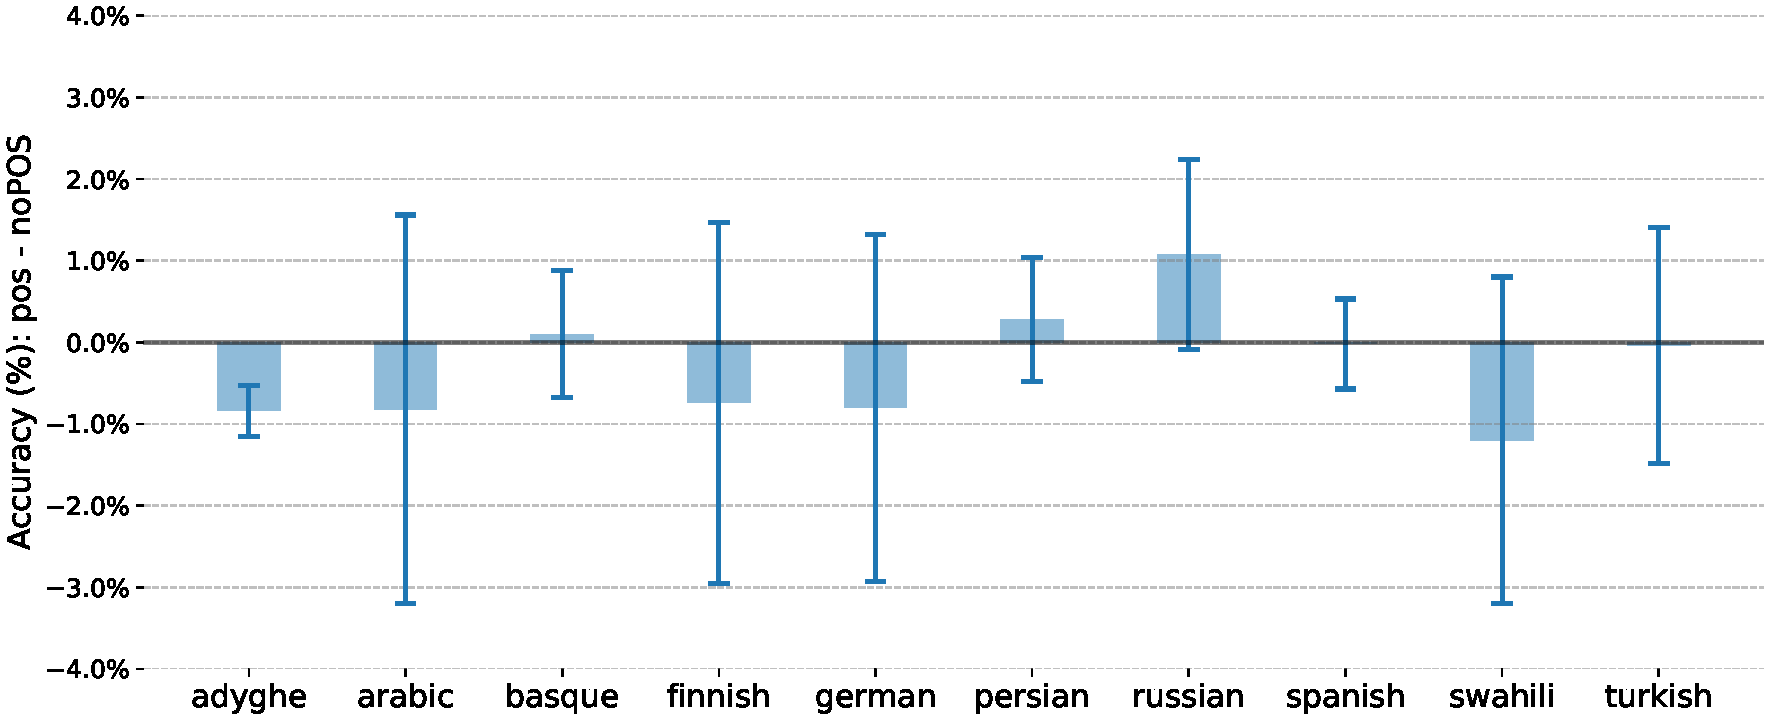
\includegraphics[width=34em]{figs/pos_2018data.pdf}
    \caption[SIGMORPHON Reinflection with/out POS Tags]{The difference in accuracy with/out POS on the reinflection task with SIGMORPHON languages. Negative scores indicates that adding POS tags improves results. The bar shows the mean of the differences and lines indicate the range of the mean plus or minus the standard deviation.}
    \label{fig:sigreinfl}
\end{figure}

\begin{figure}[!tb]
    \centering
    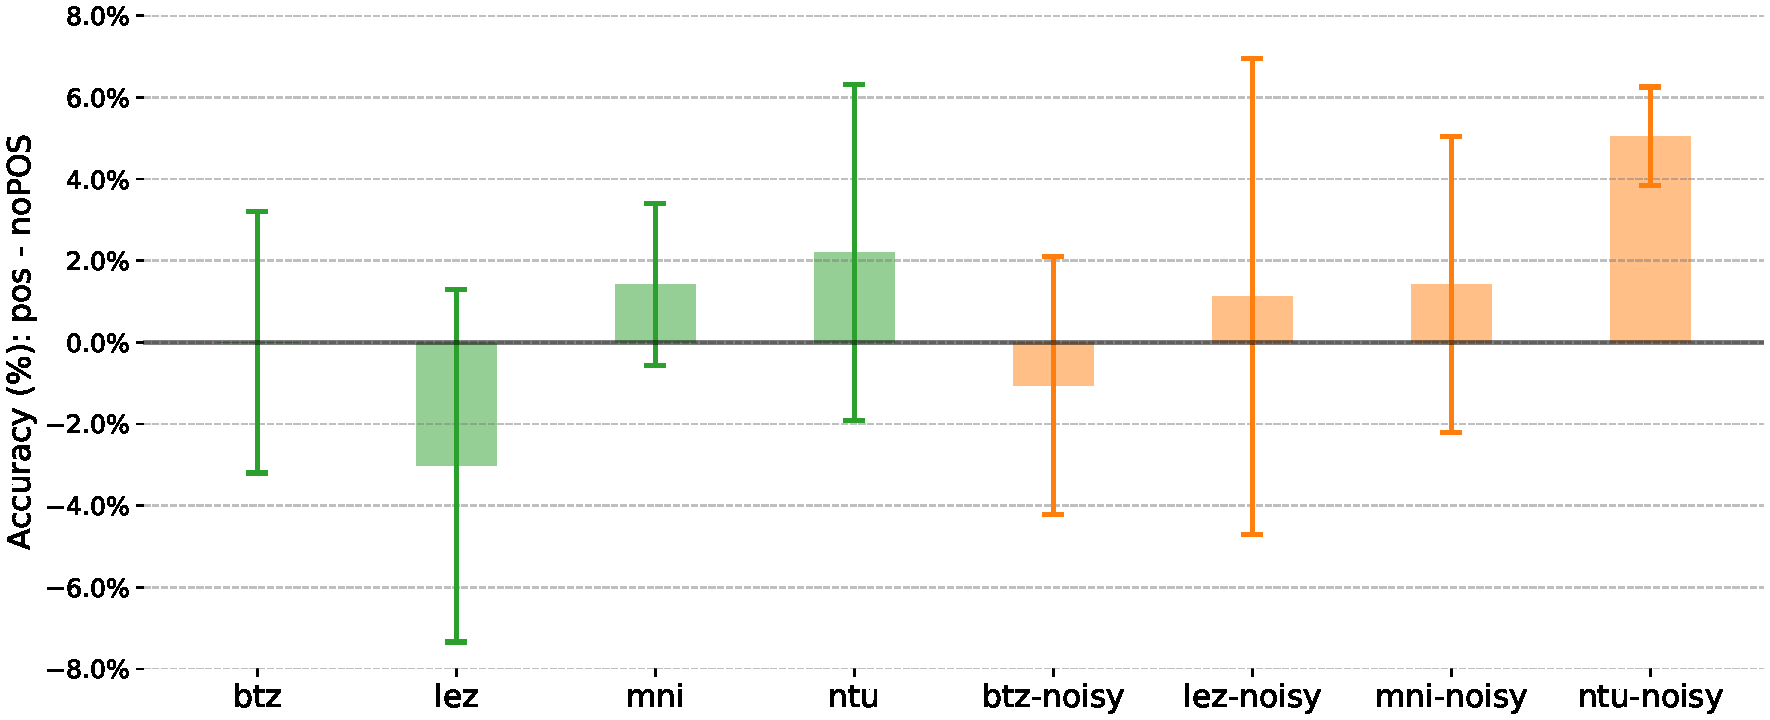
\includegraphics[width=41em]{figs/pos_igtdata.pdf}
    \caption[IGT Reinflection with/out POS Tags]{The difference in accuracy with/out POS on the reinflection task with cleaned and noisy field data. Negative scores indicates that adding POS tags improve results. The bar shows the mean of the differences and line indicates the range of the mean plus or minus the standard deviation.}
    \label{fig:igtreinfl}
\end{figure}


Five reinflection models with random seeds were trained on each data set. All models were trained twice, once with and once without POS tags on the input. Crosswise pairs were compared by subtracting the results with POS tags from the results without POS, giving 25 accuracy scores per language. Figures \ref{fig:sigreinfl} and \ref{fig:igtreinfl} show the average and range of differences between the two.  

The range of differences shows that POS tags do not have a consistently positive or negative impact. Only two languages show a clear tendency to be impact in one way. In Nat\"ugu, POS tags improve accuracy while in Adyghe, they decreases accuracy. 

The average difference in accuracy on any data set is rarely more than 1 percentage point. As the data becomes less polished, the impact of POS tags increases slightly and the range of differences grows noticeably. The largest average difference (~5 percentage points) seen in the noisy data from field IGT. This indicates that time invested in polishing existing IGT data may give a better return than time spent on POS-tagging. For the SIGMORPHON languages, the largest mean difference is barely over 2 points and for the clean IGT-extracted data the largest mean difference is about 3 points. 
%of higher accuracy \textit{without} POS tags. 

%The Lezgi data presents an anomaly among the field data sets because it is the only where accuracy reduces on the clean data. There was significant variation in accuracy across the five models of the Lezgi clean data without POS tags. This may indicate that POS tags might sometimes be helpful for this heavily agglutinative language, but the difference is not large enough to say this with certainty and the test should be repeated on related Nakh-Daghestanian languages.
%LOOK AT LEZGI DATA


\section{Discussion}
\label{sec:posdiscussion}

The number of language we used is not large but a few general observations can be made. For both tasks the impact made by the presence or absence of POS tags is minimal. 
Still best results with a small corpus are achieved when either all or no tokens are POS-tagged, at least for segmentation and glossing. This suggests that having a completely tagged corpus is better than an incompletely tagged corpus, so perhaps limited annotation time might be better spent on more segmentation and glossing. 

The size or specificity of the tag set may make a difference in the impact of POS tags. When comparing the tag sets in the SIGMORPHON data and the IGT from fieldwork, the difference in the number of lexical categories is significant. The SIGMORPHON data sets have at most three: noun (\textsc{n}), verb (\textsc{v}), and adjective (\textsc{adj}). The IGT corpora have larger tag sets; for example, they may have tags for both finite verb form (\textsc{vf}) and non-finite forms (\textsc{vnf}). The smallest IGT tag set has six categories (Manipuri). That is twice as many POS tags as the SIGMORPHON languages, but still much smaller than the other corpora, which have over 20 unique tags.  However, the difference in results cannot be definitely attributed to tag set size. The IGT tag sets are larger because the goal of descriptive work is to discover fine-grained categories, whereas the Unimorph data use more general categories which are common for language learning material or general dictionaries. Similar fine-grained distinctions appear in the Penn TreeBank tag set, are are presumably useful for NLP tasks.
%Descriptive labels may represent distinct lexical categories in a language, but may also simply indicate specific inflectional or derivational forms or reflect semantic classes with no morphological differences, like proper nouns (\textsc{nprop} and common nouns in English. 
Future work could re-tag IGT with more general categories to test how the size and specificity of POS tags on small corpora impact these tasks. This could be fruitful area of research because it might help us predict the usefulness of another linguistic category: the category of morphemes. Morpheme-level categories are similar to POS tags but tagged for individual morphemes. Interestingly, morpheme categories generally take higher priority than word-level tags in documentary and descriptive linguists and are therefore more often available in field data.

%The tag sets provided by annotators in the field data included tags such as <NotSure> or <AttachesToAnyCategory>. This means that less POS tags are actually available than shown in Table \ref{tab:data}. What happens if filtered?

%Consistency of annotation may be significant. Metrics for annotation quality should be devised so that . Linguists need to know what as they start what is important to focus on in order to gain best automated help later. 

Finally, although a consistent impact by POS tags cannot be seen on morphological analysis across corpora, some corpora did see a slight impact from the presence or absence of POS tags. Sometimes better results were had by removing POS tags, sometimes by adding them. Reinflection in Adyghe and the ``clean'' version of Lezgi data tend to benefit by removing POS tags while Persian, Russian, and the noisy version of Nat\"ugu generally have more accurate results with POS tags. In segmentation and glossing, Alas and Lamkang show in some settings nearly .1 points difference when POS tags are added and removed, respectively. With these trends, a more interesting question for these corpora becomes ``When are POS tags helpful?'' and this should be explored further. 


\section{Conclusion}

We conclude that the presence or absence of POS tags does not have a significant impact on two morphological analysis tasks: segmentation and glossing, or reinflection. There is no clear advantage from doing POS-tagging on low-resource data. In segmentation and glossing, the greatest average difference is a loss of .09 F$_1$-score when a large POS tag set is added to a small field corpus. In reinflection, the overall tendency, though slight, is that accuracy actually decreases when POS tags are added. The greatest average difference is 1.2 points of accuracy for published data, 2.2 points for unpublished ``clean'' data, and 5 points for unpublished noisy data.

We hypothesize that POS tags do not have a significant impact on these tasks because the information provided by POS tags is implicitly learned. These are not only two tasks where POS tags could be leveraged for low-resource languages and we cannot make a definitive statement regarding the impact of POS tags in other NLP tasks with low-resource languages, particularly ones that more syntactic or semantic in nature. However, it does bring into question whether the development of POS taggers and POS tagging should be given the priority they have assumed. This needs to be methodically tested. 

Future work should explore how other NLP tasks are impacted by POS tags. The results might influence workflow priorities for documentary and descriptive linguists who want to receive/give benefit from/to NLP. When a sophisticated POS tag set and POS taggers are available for a language, then leveraging POS tags is a trivial matter. However, as NLP expands into a broader range of languages, the usefulness of POS tags may become an important question because documentary and descriptive linguistics does not currently place a high priority on lexical categories. Discovering a language's lexical categories requires a detailed understanding of the language's syntax--something linguists do not always possess in the early stages of describing a new language. 

%However, if NLP hopes to expand its reach, then the first question should still be the one we ask here: ``What is the impact of (not) having POS tags?''. If the impact is high, then we may want to focus on interdisciplinary dialogue that could basically request field linguists to put higher emphasis on POS tagging. This would need to be accompanied with clarification of how this might also benefit their work. A better approach, however, would be to collaboratively discover and tag another type of information that might be just as or more helpful to NLP and hold more theoretical interest to some documentary and descriptive linguists, such as grammatical relations or thematic roles.


%If POS tags are not helpful in learning morphological patterns, what does this mean for questions about POS being a universal property of language?

%Testing the assumption that POS tags are useful in low-resource settings is an interesting question because documentary and descriptive linguistics, which create annotated resources in new languages, does not put as high a priority on identifying lexical categories as NLP does. 
%POS-tagging is rarely, if ever, mentioned as part of the language documentation workflow 
%and if POS tagging is prioritized, then it is usually because the project's short-term goals will directly benefit from it, such as allowing descriptive work to focus on verb tenses in narrative discourse.
%For example, a linguist studying the salience of verb tenses in narrative discourse may prioritize lexical categories identification so that early analytic tasks such as morpheme segmentation and glossing can be focused on the verbs. 
%Several other tasks are prioritized over POS tagging, including translation, morpheme segmentation and glossing, lexicon building, morphological inflectional paradigm elicitation, and even sketching a full grammar \citep{bird_machine_2012}. This mismatch of priorities presents a potential conflict for NLP work with low-resource languages or for leveraging NLP systems to assist linguistic analysis of under-documented languages. 
%, even a similar tagging process for morphemes (not words) .
%which is similar to POS tagging but tags morphemes, not words. Without a good knowledge of the language's structure, it may not be possible to decipher POS information from the morpheme tags.  

%It makes little sense to introduce one more task to already overburdened field linguists if the task holds little promise to improve or speed their later work or the development of NLP. This is particularly weighty when we consider how complicated the task can be. 
 
%Skimming through the head words of an English dictionary, for example, shows that parts of speech are not uniquely or consistently distinguished except for (most) adverbs which are marked with ``-ly''.

%Four---Alas, Lezgi, Manipuri, and Nat\"ugu---IGT have a significant number of word-level POS tags and will be used in the inflection experiment. Arapaho and Tsez have ``POS'' tags only for morphemes and Lamkang has a very small amount of word-level POS tags, so these languages will be used only for the segmentation and glossing experiment.
